\documentclass[dvipdfmx, 11pt, twocolumn]{jsarticle}

% --- パッケージの読み込み ---
\usepackage[T1]{fontenc}
\usepackage{mathrsfs}
\usepackage[top=10truemm,bottom=20truemm,left=15truemm,right=15truemm]{geometry} % 余白の設定
\usepackage{amsmath,amssymb} % 数式用
\usepackage{bm}              % 太字ベクトル用
\usepackage[dvipdfmx]{graphicx} % 画像読み込み用 (Overleaf等の場合は [dvipdfmx] を外しても動くことが多いです)
\usepackage{comment}
\usepackage[font=scriptsize]{caption}
\usepackage{physics}
\usepackage{url}             % URL表示用
% \usepackage{times}           % 英数字のフォントをTimes系に
% \usepackage{newtxtext,newtxmath} % より物理学会風のフォント設定（数式含む）

% --- タイトル設定 ---
% 論文タイトル
% \title{\Large \bfseries Bose凝縮による超伝導状態の再現とギャップ方程式の数値解析}

% 著者名・所属
% \author{   
%    \normalsize 理論物理学研究室\\
%    \normalsize 2213100\ 田中 響\\
%    \normalsize 指導教員：長田 剛\\
% }
% \date{\vspace{-5mm}} % 日付を出さない場合は空欄

% --- 本文開始 ---
\begin{document}

% タイトル部分の出力
% \maketitle
\twocolumn[
\begin{center}
    % タイトル（中央揃え）
    \vspace{0mm} % 上の余白調整
    {\Large \bfseries Bose凝縮による超伝導状態の再現とギャップ方程式の数値解析}
    \vspace{0mm} % タイトルと著者の間の余白
\end{center}

\begin{flushright}
    % 著者情報（右揃え）
    % 文字サイズを少し大きく（お好みで）
    \normalsize 理論物理学研究室\\
    \normalsize 2213100\ 田中 響\\
    \normalsize 指導教員：長田 剛
\end{flushright}
\vspace{1mm} % 本文との間の余白
]
% セクションのフォントサイズ等を微調整（必要に応じて）
\section{はじめに}
超伝導研究の歴史は1911年Kamerligh-Onnesが液体ヘリウムを用いて水銀を冷却したこところ、4.2Kで突然抵抗が零になる現象が発見されたことにより始まった。その特異的な現象は相転移現象によるものだと考えられ研究が進み、超伝導体内部で磁場が排除されるMeissner効果や、比熱の不連続性などの現象が確認された。そして1957年Bardeen,Cooper, Schriefferの三人が微視的に超伝導状態を説明するBCS理論を提唱し、それが見事に実験結果と一致し成功を収めた。本研究ではBCS理論に倣い、二電子から構成されるCooper対がBose凝縮を起こすことを仮定し具体的なモデルを用いて超伝導状態の再現を行い、ギャップ方程式の数値解による考察を行った。
\section{超伝導状態の現象論}
\subsection{London理論}
    抵抗を受けずに運動する超伝導電子がNewtonの運動方程式に従うと仮定しMaxwell方程式を用いると
    \begin{align}
        \mu_0\bm{\nabla} \times \bm{j}_S  + \frac{1}{\lambda_L^2} \bm{B} = 0
    \end{align}
    が導かれる。これをLondon方程式という。ここで$\bm{j}_S$は超伝導電子からなる電流であり、$\lambda_L$は磁場の侵入長とよばれる定数である。さらにMaxwell方程式を用いると
    \begin{align}
        \nabla^2 \bm{B} - \frac{1}{\lambda_L^2} \bm{B} =0
    \end{align}
    磁束密度に関して閉じた微分方程式が得られる。この方程式は磁場の空間的な減衰を表し、Meissner効果が図1に示す様に再現される。
    \begin{figure}[htbp]
        \centering
        \includegraphics[width=50mm]{london_16x9_wallpaper.png} % 画像ファイル
        \caption{球形超伝導体に一様な磁場を印加した際の磁力線と電流分布}
        \label{fig:result}
        \vspace{-10mm}
    \end{figure}
\begin{comment}
\subsection{量子力学との類似性}
    London理論からベクトルポテンシャルに比例した電流が得られる。この事実は量子力学における電流と類似していることが分かる
    \begin{align}
        \bm{j} = \frac{e\hbar}{2mi}\left( \psi^* \bm{\nabla} \psi - \psi \bm{\nabla} \psi^* \right) - \frac{e^2}{m}|\psi|^2 \bm{A}
    \end{align}
    しかしこの表式はLondon理論とでは
    \begin{align}
        &\text{・多粒子の電流ではなく一粒子に対する電荷の流れ} \notag \\
        &\text{・波動関数の勾配項が存在する} \notag 
    \end{align}
    の点で異なる。しかし、もし「多数の粒子が一粒子のようにふるまい、波動関数の勾配が無視できるほど小さくなる」なら量子力学的な電流はLondon理論の電流と一致する。さらに実験から超伝導電流を担う電子の電荷が$2e$であるこが知られており、超伝導状態は二つの電子がBose粒子を形成しBose-Einstein凝縮が起きている可能性が高いと考えられるようになった。
\end{comment}
\section{BCS理論}
\subsection{超伝導基底状態の仮定}
    現象論からの考察より超伝導基底状態を以下のように仮定する
    \begin{align}
        &\text{・二つの電子が束縛状態となりCooper対を形成}\notag \\
        &\text{・全てのCooper対が同じ状態に凝縮している} \notag \\
        &\text{・等方的なs波スピン一重項のCooper対を形成} \notag 
    \end{align}
    したがって、超伝導基底状態の波動関数は、粒子の生成演算子を$\hat{c}^\dagger$とすると
    \begin{align}
        \ket{\Psi_{\textbf{BCS}}} := \prod_{\bm{k}}\left( u_{\bm{k}} + v_{\bm{k}}\hat{c}_{\bm{k}\uparrow}^\dagger \hat{c}_{-\bm{k}\downarrow}^\dagger \right) \ket{0}
    \end{align}
    とかける。ここでパラメータ$u_{\bm{k}},v_{\bm{k}}$は凝縮波動関数$\phi(\xi_1,\xi_2)$のフーリエ成分$\phi_{\bm{k}}$として
    \begin{align}
        u_{\bm{k}} := \frac{1}{\sqrt{1+|\phi_{\bm{k}}|^2}} ,\quad
        v_{\bm{k}} := \frac{\phi_{\bm{k}}}{\sqrt{1+|\phi_{\bm{k}}|^2}}
    \end{align}
    と定義した。Fermiエネルギーを基準とした一粒子エネルギーを$\xi_{\bm{k}}$としCooper対の相互作用を考慮したハミルトニアンは
    \begin{equation}
        \hat{H} := \sum_{\bm{k}}\sum_{\alpha} \xi_{\bm{k}} \hat{c}^\dagger_{\bm{k}\alpha} \hat{c}_{\bm{k}\alpha} + \sum_{\bm{k}}\sum_{\bm{k}'} U_{\bm{k}\bm{k}'} \hat{c}_{\bm{k}\uparrow}^\dagger \hat{c}_{-\bm{k}\downarrow}^\dagger \hat{c}_{-\bm{k}'\downarrow}\hat{c}_{\bm{k}'\uparrow}
    \end{equation}
    となる。以上から
    \begin{align}
        &\text{・超伝導-常伝導相転移} \notag \\
        &\text{・比熱の不連続性}\notag
    \end{align}
    を導くことができれば仮定の妥当性が確認されると考えられる。
\subsection{超伝導励起状態}
    有限温度でのふるまいを調べるために基底状態からの励起を考える。超伝導状態の励起はBogoliubov-Valatin(B-V)演算子$\hat{\gamma}^\dagger,\hat{\gamma}$で表される。
    \begin{align}
        \left[ 
        \begin{matrix}
            \hat{\gamma}^\dagger_{\bm{k}\uparrow}\\
            \hat{\gamma}_{-\bm{k}\downarrow} \\
            \hat{\gamma}^\dagger_{-\bm{k}\downarrow}\\
            \hat{\gamma}_{\bm{k}\uparrow}
        \end{matrix}
        \right] =
        \left[
        \begin{matrix}
            u_{\bm{k}}^*&-v_{\bm{k}}^*&0&0\\
            v_{\bm{k}}&u_{\bm{k}}&0&0\\
            0&0&u_{\bm{k}}^*&v_{\bm{k}}^*\\
            0&0&-v_{\bm{k}}&u_{\bm{k}}
        \end{matrix}
        \right]
        \left[
            \begin{matrix}
                \hat{c}^\dagger_{\bm{k}\uparrow}\\
                \hat{c}_{-\bm{k}\downarrow} \\
                \hat{c}^\dagger_{-\bm{k}\downarrow}\\
                \hat{c}_{\bm{k}\uparrow}
            \end{matrix}
        \right]
    \end{align}
    平均場近似を用いたハミルトニアンは
    \begin{align}
        \hat{\mathcal{H}}_{\textbf{BCS}} := W_0^S + \sum_{\bm{k}} E_{\bm{k}}(\hat{\gamma}^\dagger_{\bm{k}\uparrow} \hat{\gamma}_{\bm{k}\uparrow} + \hat{\gamma}^\dagger_{-\bm{k}\downarrow} \hat{\gamma}_{-\bm{k}\downarrow} ) 
    \end{align}
    となる。BV演算子で励起される場は自由粒子の様にふるまう準粒子となっており、ボゴロンとよばれる。ボゴロンの励起エネルギーは
    \begin{align}
        E_{\bm{k}} = \sqrt{\xi_{\bm{k}}^2 + \Delta_{\bm{k}}^2}
    \end{align}
    で与えられ、この励起に必要な最小のエネルギーは$2\Delta_{\bm{k}_F}$必要なことから$\Delta_{\bm{k}}$はギャップ関数と呼ばれる。
\subsection{ギャップ方程式}
    ギャップ関数は以下の方程式を自己無撞着に解くことで求めることができ、これをギャップ方程式という
    \begin{equation}
        \Delta_{\bm{k}}(T) = -\sum_{\bm{k}'} U_{\bm{k}\bm{k}'}  \frac{\Delta_{\bm{k}'}(T)}{2\sqrt{\xi_{\bm{k}'}^2 + \Delta_{\bm{k}'}^2(T)}} \tanh \frac{\beta E_{\bm{k}'}}{2}
    \end{equation}
    パラメータ$u_{\bm{k}},v_{\bm{k}}$もギャップ関数を用いて表すことができ、超伝導状態はギャップ関数を定めることにより一意的に記述される。
\section{数値計算結果と考察}
\subsection{ギャップ関数}
    ギャップ方程式を実際に解くために本研究ではFermi面付近の電子対に相互作用が働くモデルを採用し以下のようにポテンシャルを設定した。
    \begin{align}
        U_{\bm{k}\bm{k}'} = -U_0 \theta(\hbar\omega_D - |\xi_{\bm{k}}|) \theta(\hbar\omega_D - |\xi_{\bm{k}'}|)
    \end{align}
    ここで、$\theta(x)$はステップ関数であり、カットオフエネルギーをDebyeエネルギー$\hbar \omega_D$とした。実際にポテンシャルを代入するとギャップ関数は
    \begin{align}
        \Delta_{\bm{k}}(T) = \Delta(T)\ \theta(\hbar \omega_D - |\xi_{\bm{k}}|)
    \end{align}
    となり、ギャップ方程式は
    \begin{align}
        1  =  U_0{\sum_{\bm{k}'}}'   \frac{1}{2\sqrt{\xi_{\bm{k}'}^2 + \Delta^2(T)}} \tanh \frac{ \sqrt{\xi_{\bm{k}'}^2 + \Delta^2(T)}}{2k_B T} 
    \end{align}
    となる。ただし、$\sum'$は$|\xi_{\bm{k}}|\le \hbar \omega_D$を満たすFermi面近傍の波数に対する和を表す。数値計算により求めたギャップ関数の温度依存性の結果は図2に示す
\subsection{比熱}
    また、比熱は以下で与えられる
    \begin{equation}
        C = 2\sum_{\bm{k}}  \frac{e^{\beta E_{\bm{k}}}}{(e^{\beta E_{\bm{k}}}+1)^2} \left\{ k_B \beta^2 E_{\bm{k}}^2 - \frac{1}{2k_B^2 T} 
        \frac{\partial \Delta^2_{\bm{k}}(T)}{\partial T}   \right\}
    \end{equation}
    個の比熱の温度依存性を図3に示す。
    \begin{figure}[t]
        \begin{minipage}[t]{0.48\linewidth}
            \centering
            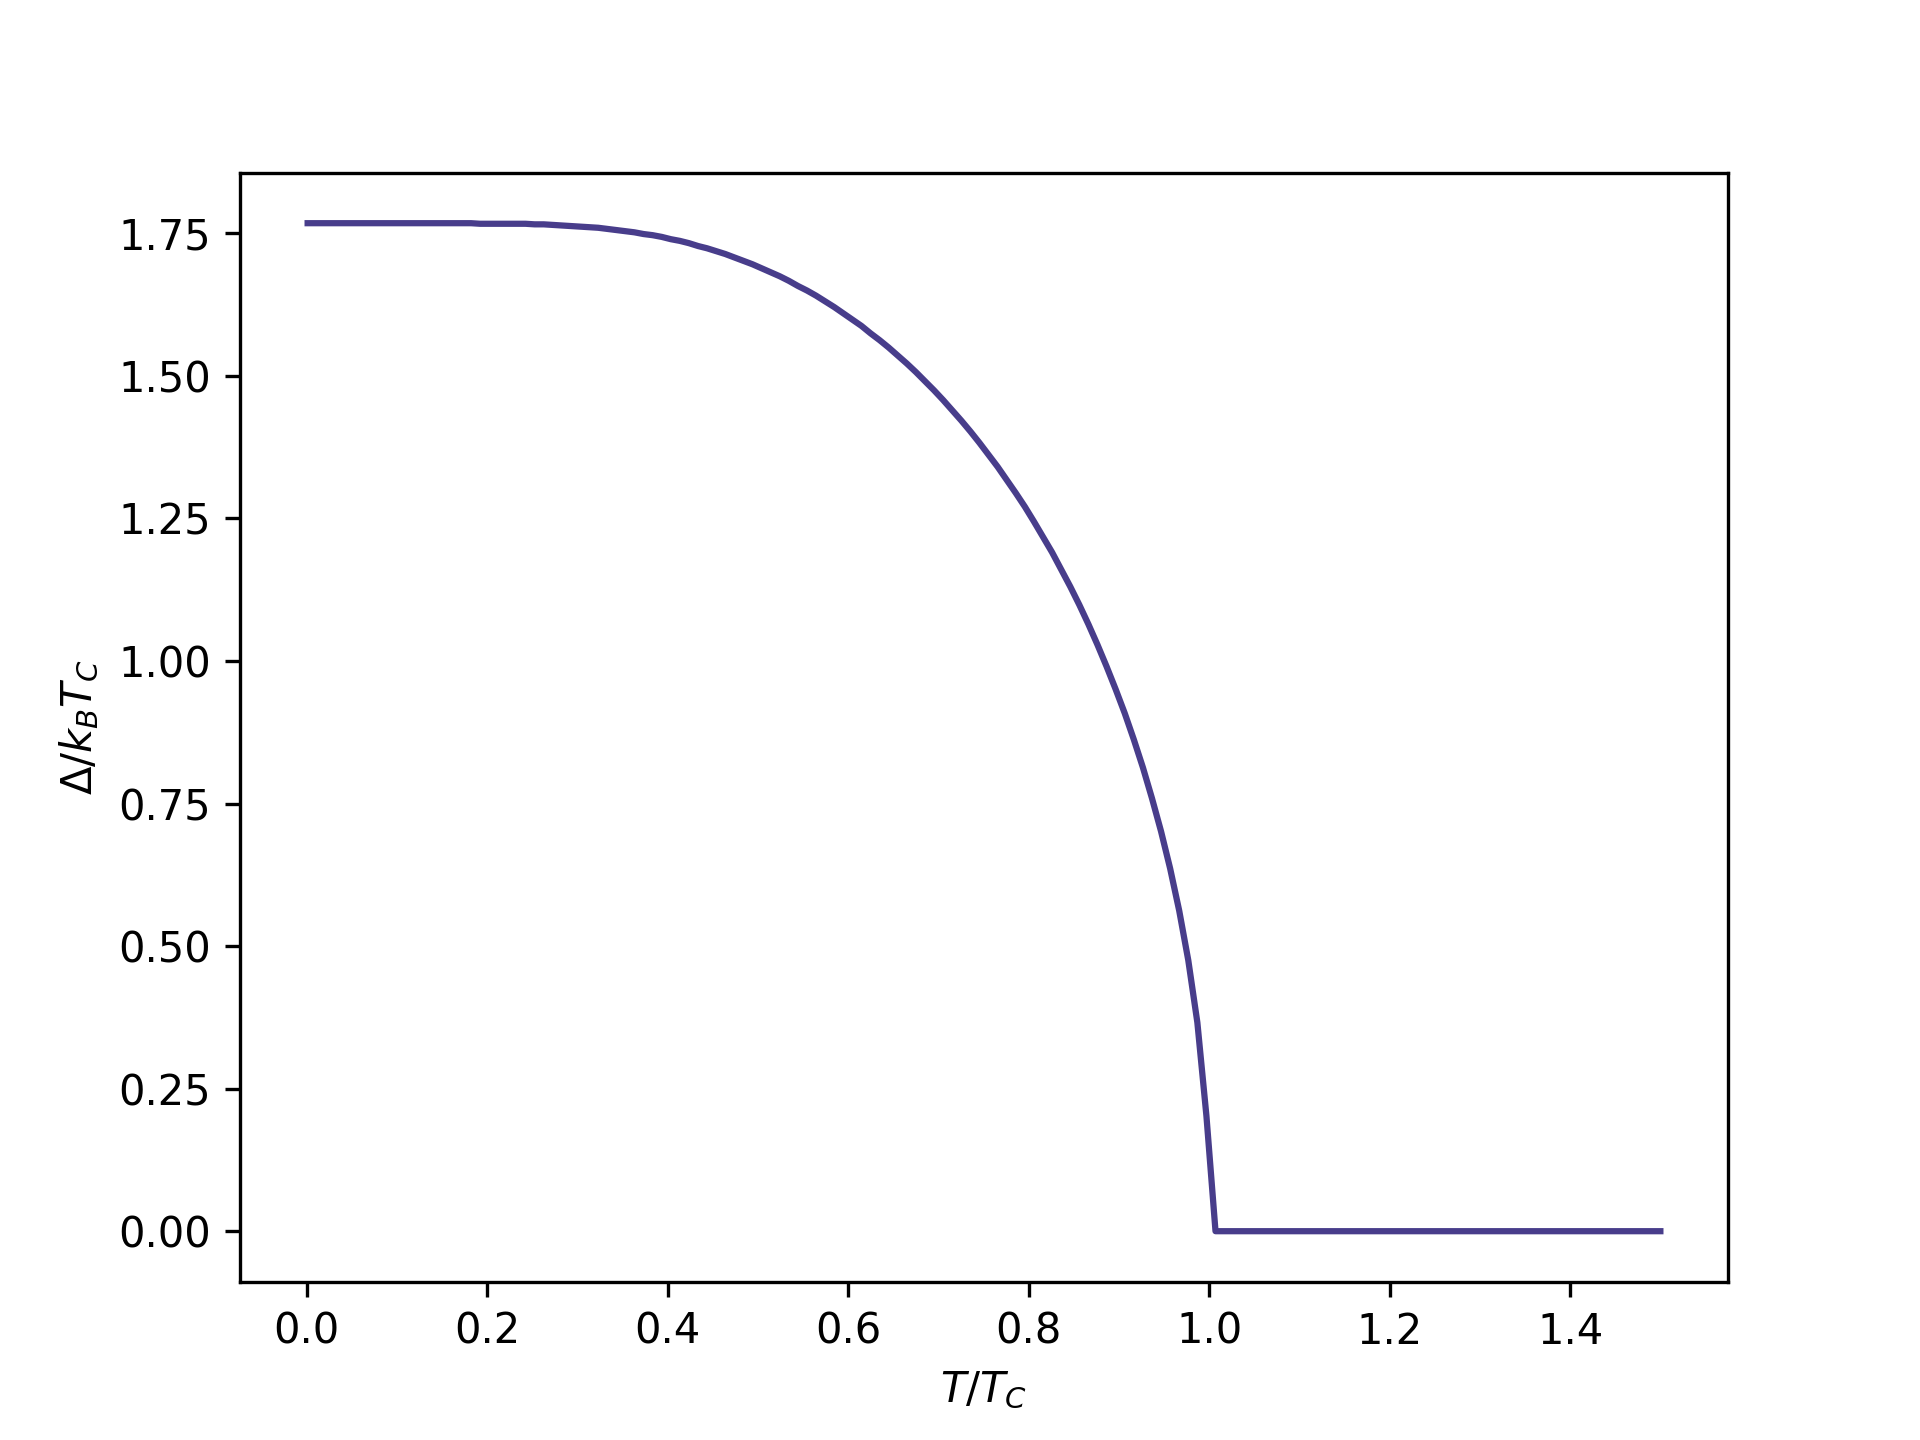
\includegraphics[width=40mm]{GapFunction.png} % 画像ファイル名を指定
            \caption{ギャップ関数の温度依存性} \scriptsize
            \label{fig1}
        \end{minipage}
        \begin{minipage}[t]{0.48\linewidth}
            \centering
            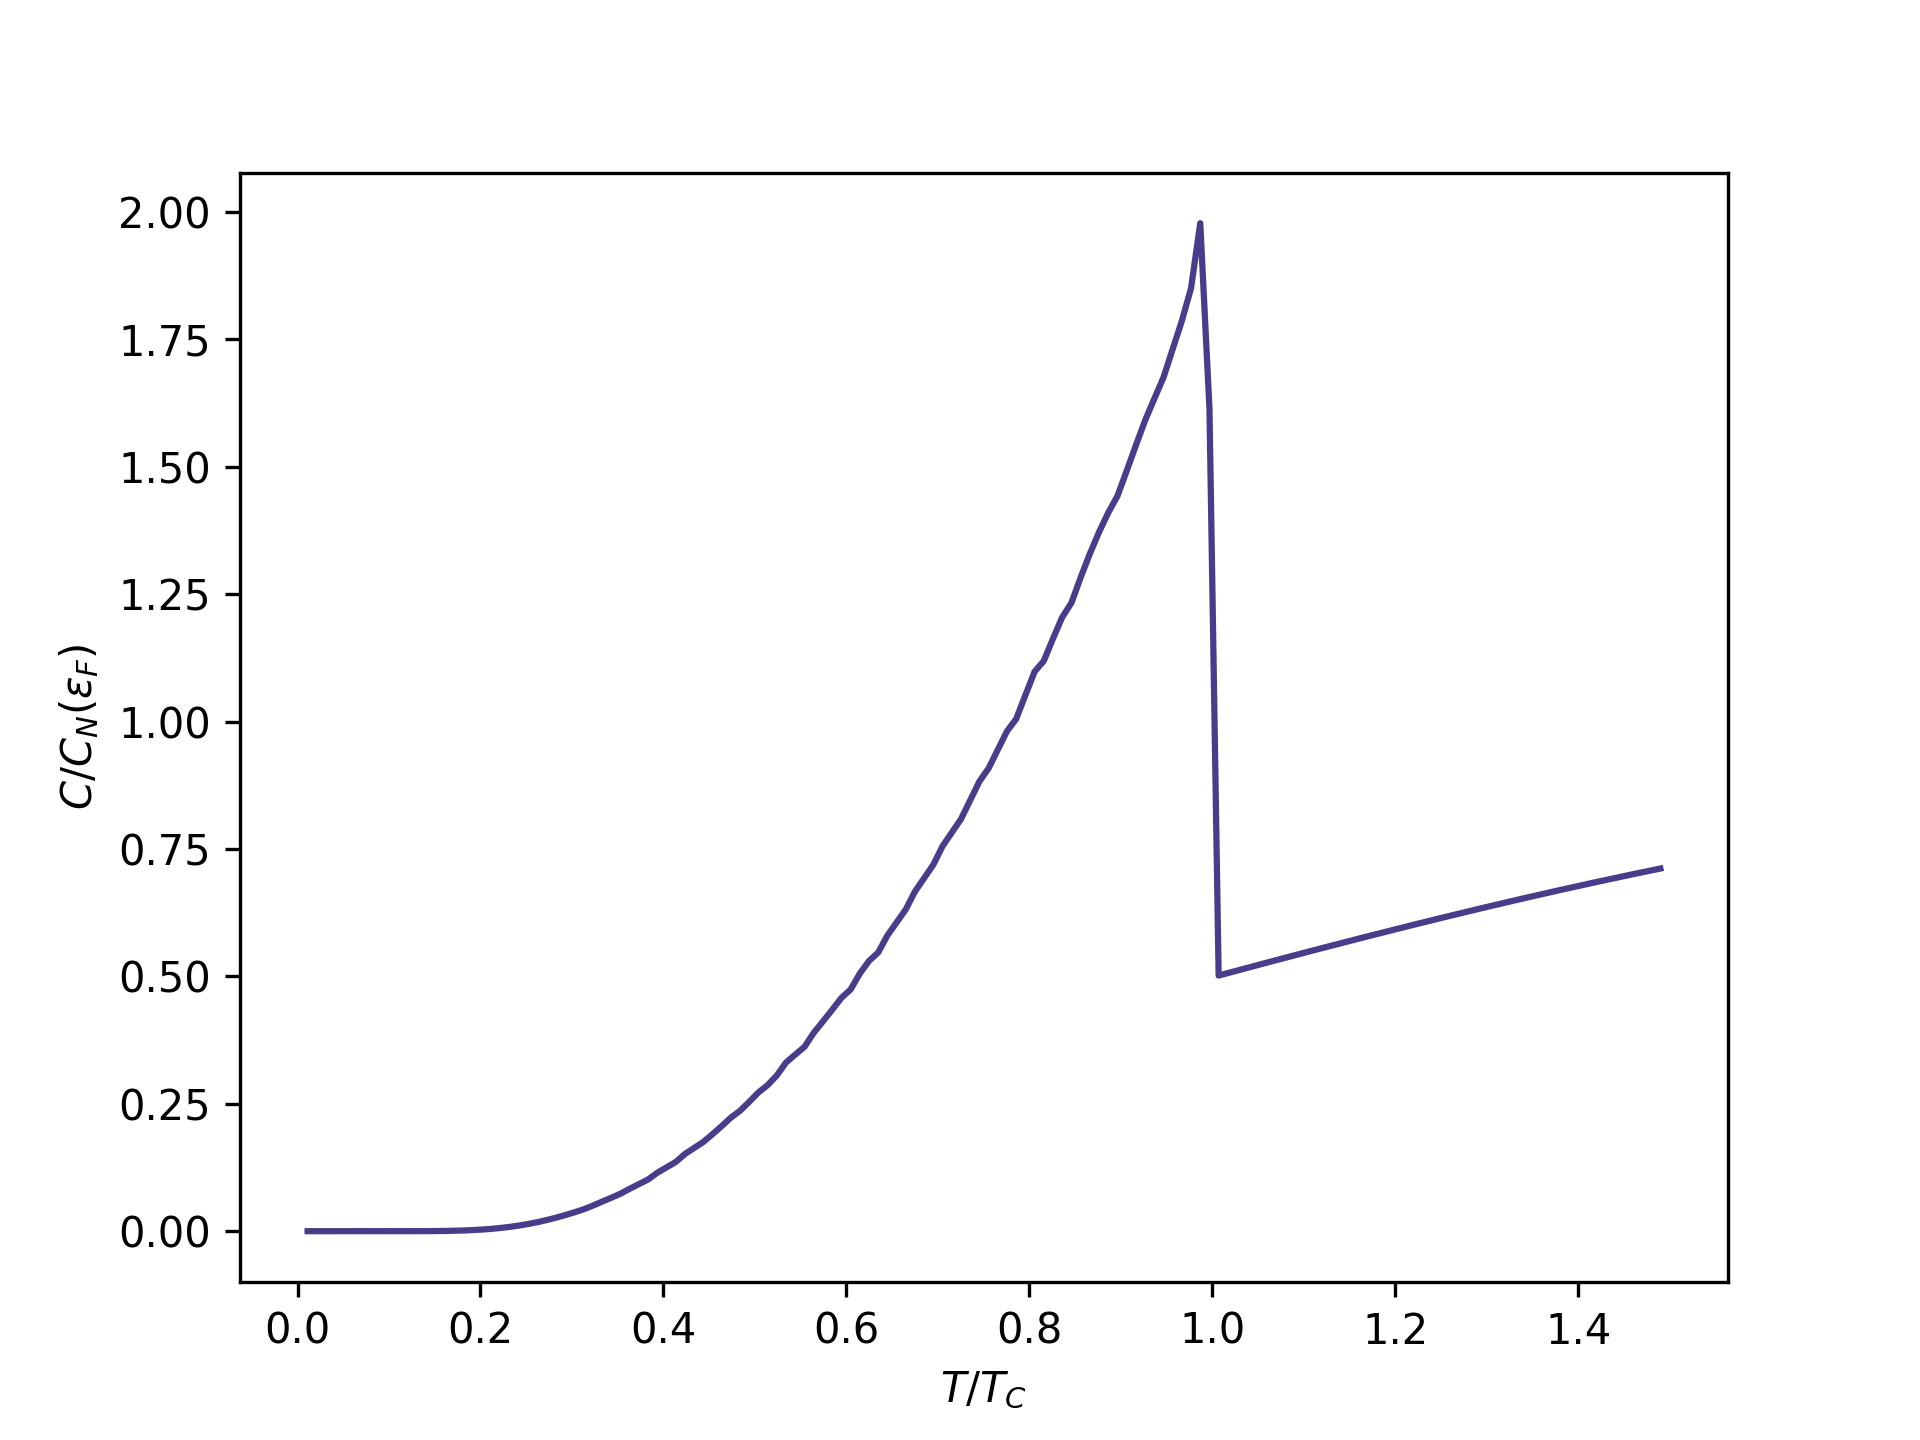
\includegraphics[width=40mm]{HeatCap.png} % 画像ファイル名を指定
            \caption{比熱の温度依存性}
            \label{fig1}
        \end{minipage}
        \vspace{-5mm}
    \end{figure}
    \begin{figure}[t]
        \begin{minipage}[t]{0.48\linewidth}
            \centering
            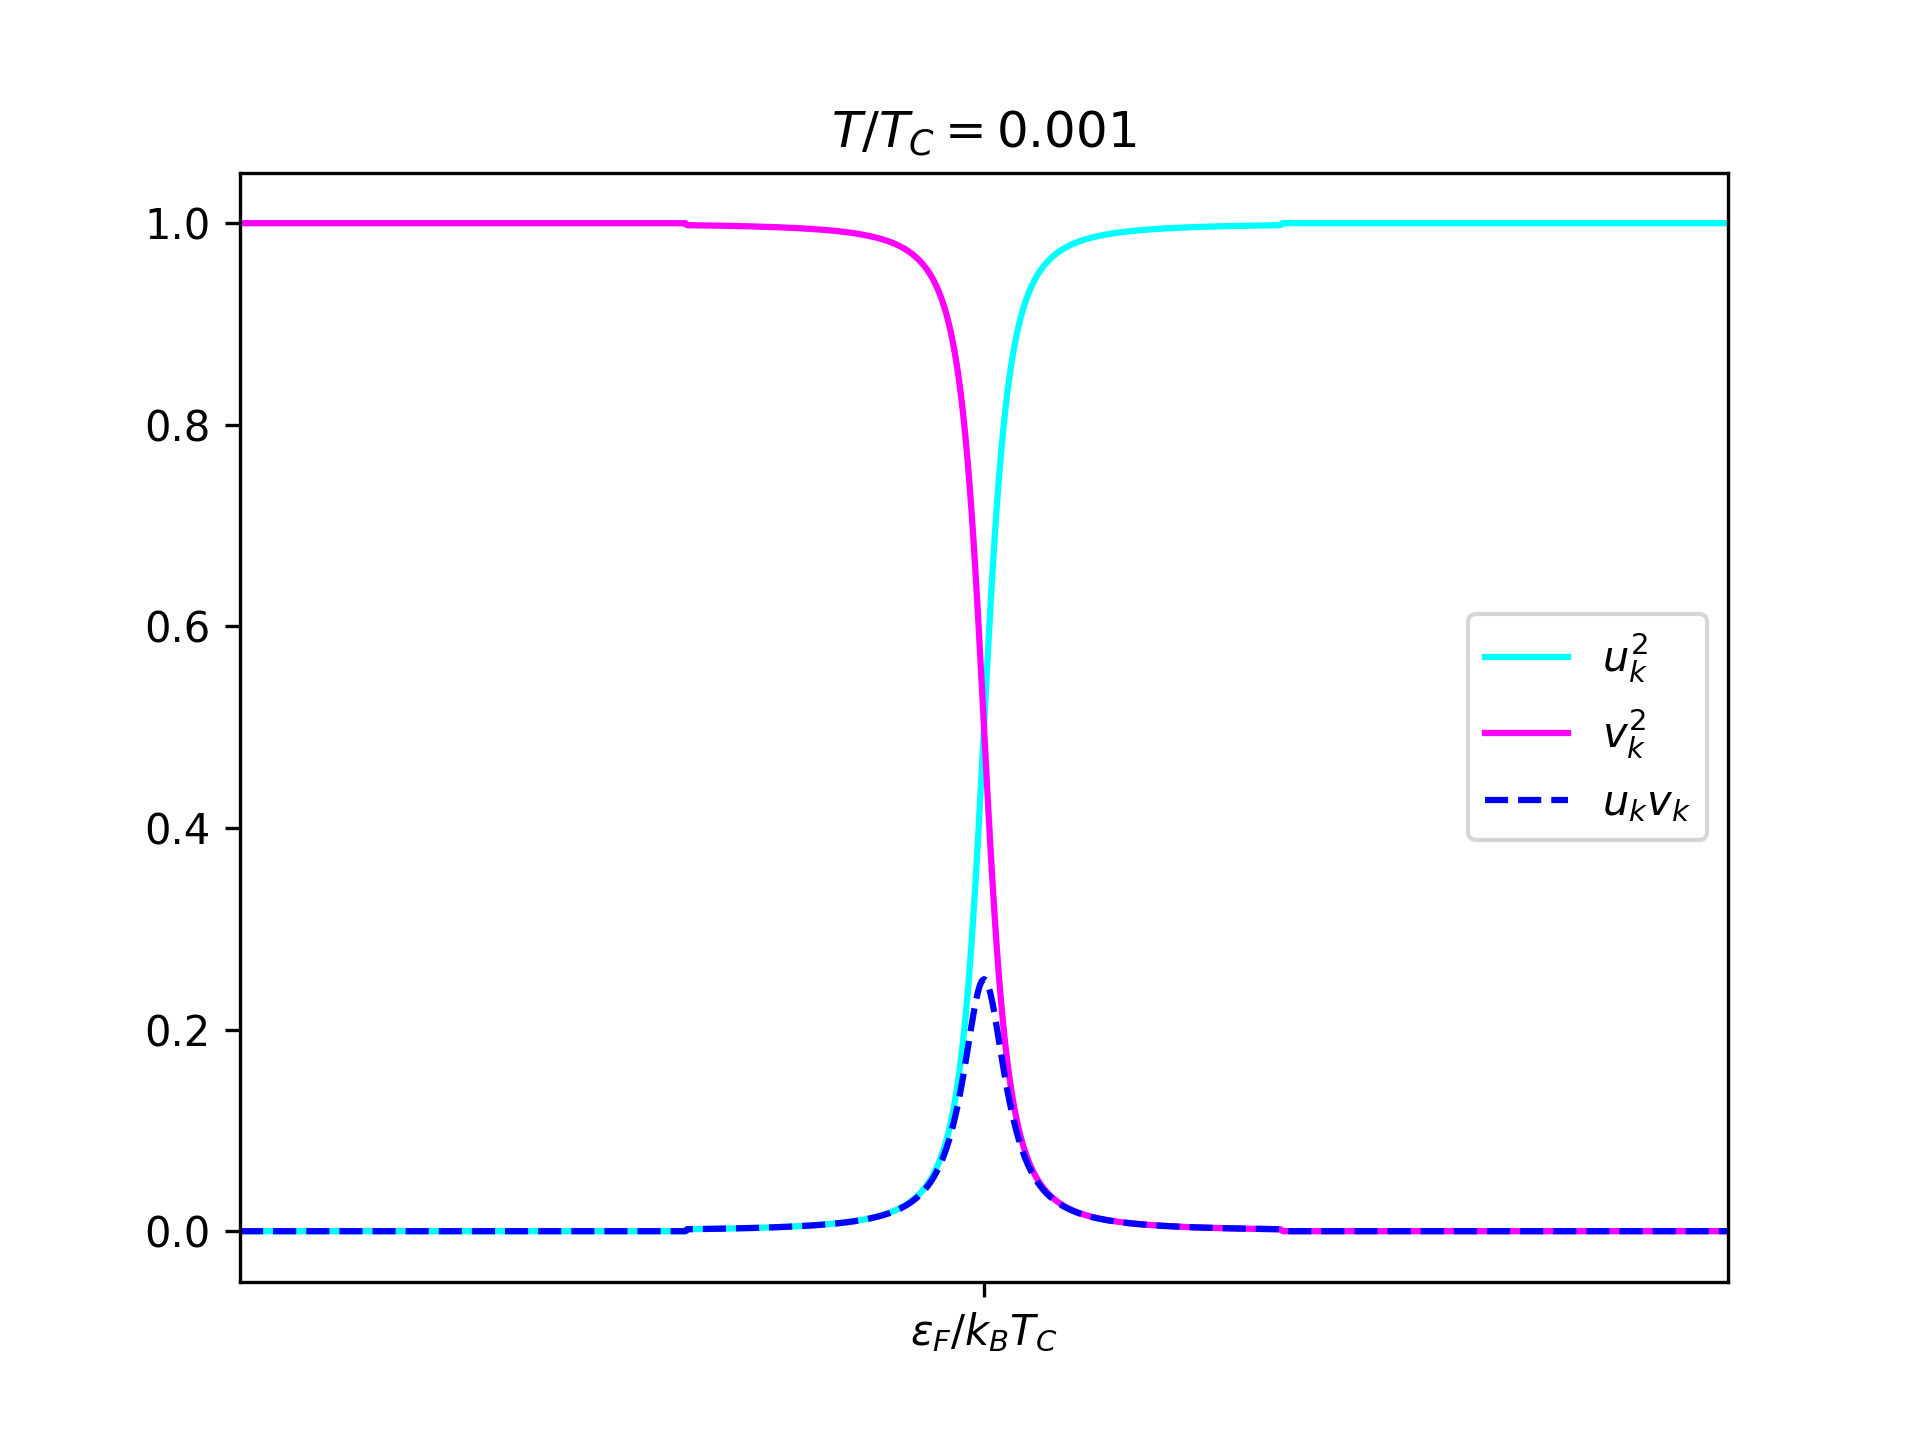
\includegraphics[width=40mm]{BCS_parameters_T=0.001.png} % 画像ファイル名を指定
            \label{fig4}
        \end{minipage}
        \begin{minipage}[t]{0.48\linewidth}
            \centering
            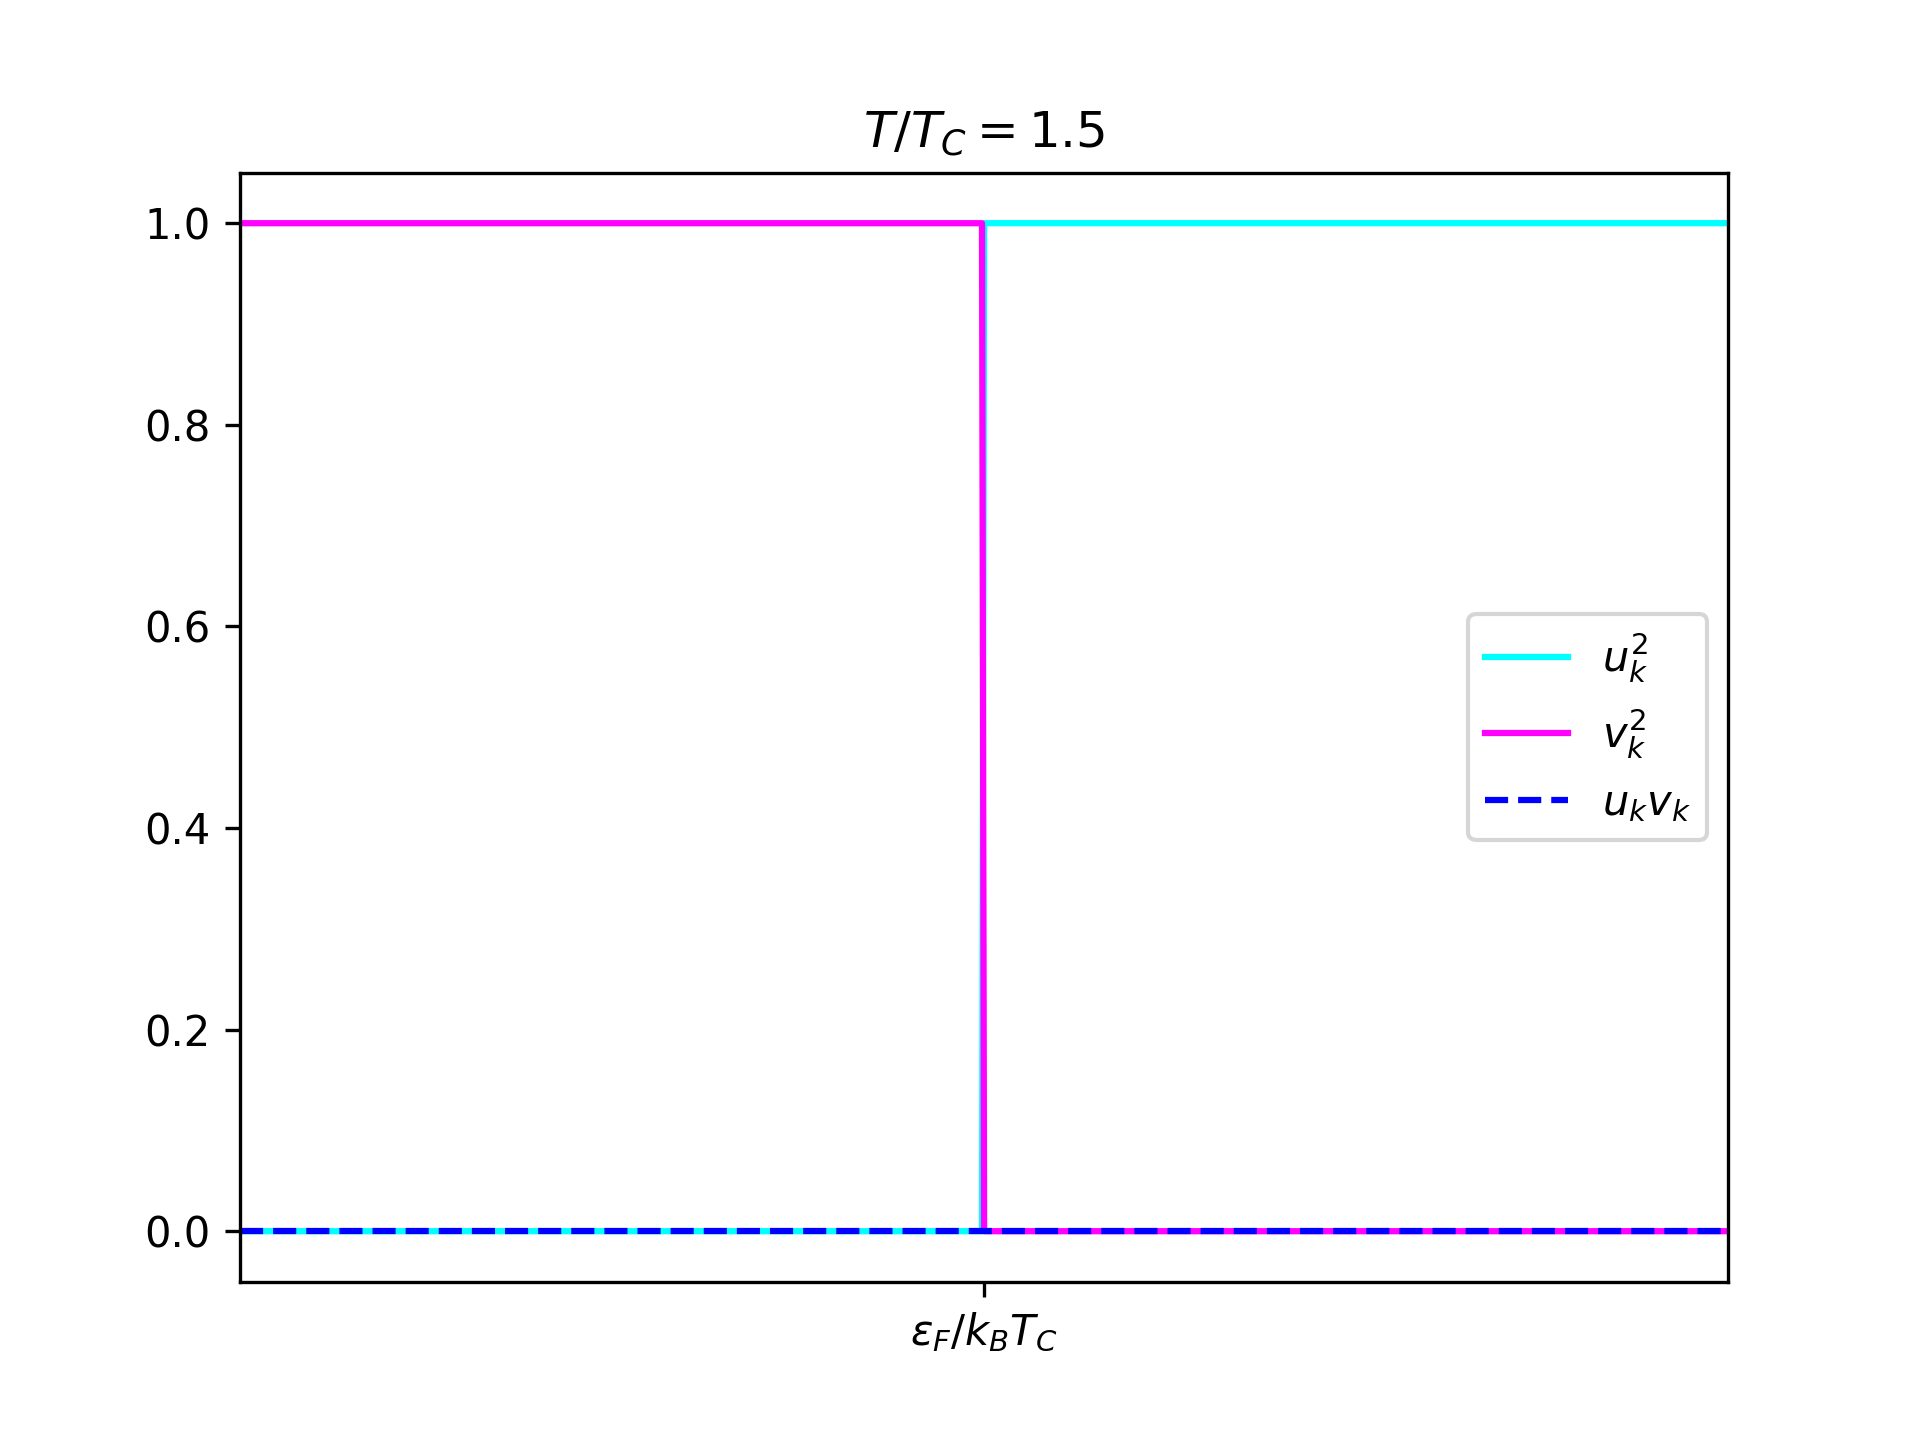
\includegraphics[width=40mm]{BCS_parameters_T=1.5.png} % 画像ファイル名を指定
            \label{fig5}
        \end{minipage}
        \vspace{-5mm}
        \caption{パラメータ$u_{\bm{k}},v_{\bm{k}}$の波数依存性}
        \vspace{-5mm}
    \end{figure}
\subsection{考察}
    さらに、図2からは系の温度が転移温度$T_C$よりも下がると急激にギャップ関数が立ち上がる相転移が起きていることが分かる。これは超伝導基底状態が
    \begin{align}
        \ket{\Psi_\textbf{BCS}} = 
        \left\{
        \begin{matrix}
            \prod_{\bm{k}}(u_{\bm{k}} + v_{\bm{k}}\hat{c}^\dagger_{\bm{k}\uparrow}\hat{c}^\dagger_{-\bm{k}\downarrow})\ket{0}&T<T_C\\
            \prod_{|\bm{k}|\le k_F}\hat{c}^\dagger_{\bm{k}\uparrow}\hat{c}^\dagger_{-\bm{k}\downarrow} \ket{0}&T_C < T
        \end{matrix}
        \right.
    \end{align}
    となっていることから、$T=T_C$において超伝導-常伝導相転移が起きていると理解することができる。また、図3から転移温度において比熱の不連続性も分かる。これらのことから、はじめに仮定した超伝導状態が再現されている。また、比熱が超伝導状態になった途端に大きくなる原因は、Cooper対の束縛状態の形成により粒子が安定な状態となり励起に必要なエネルギーが増加するためであると考えられる。
\section{まとめ}
    本研究ではBCS理論に倣い、Cooper対がBose凝縮を起こす仮定をしギャップ方程式を具体的なポテンシャルを用いて数値計算を行い、超伝導体の比熱の温度依存性などの再現を行った。結果相転移現象が数値的に確認され、仮定の妥当性も確認することができた。
% --- 参考文献 ---
% 実際の物理学会誌に近いフォーマット
\begin{thebibliography}{9}
\bibitem{ref1}丹羽 雅昭:「超伝導の基礎」東京電機大学出版局
\bibitem{ref2}北 孝文:「統計力学から理解する超伝導理論」サイエンス社
\end{thebibliography}

\end{document}